% !TEX root = ../thesis.tex
%
\chapter{Evaluation}
In this chapter, we systematically assess the performance and key characteristics of the proposed methodology.
We begin by outlining the evaluation metrics and experimental framework before presenting the results across multiple datasets.

\section{Evaluation Metrics}

\subsection{Accuracy}

\subsection{Demographic Parity}
As machine learning systems are increasingly deployed in high-stakes applications,
both neural networks and decision trees must be scrutinized for potential biases in their prediction.
This concern highlights the importance of having quantitative measures
for assessing and comparing models to ensure that they meet fairness criteria
alongside performance metrics.

Quantitative \textbf{group fairness} metrics offer a way to assess whether a machine learning model's predictions
are equitable across different groups within the population.
For PBPM, these metrics help ensure that predictions, such as the next activity or outcome in a business process,
do not favor one group over another based on sensitive attributes.
\textbf{Sensitive attributes} refer to characteristics of individuals or groups
that are typically protected by laws or ethical guidelines due to their potential to lead to biased or discriminatory treatment,
such as gender, ethnicity, age, disability status, etc.

%TODO: dem parity in discrimination aware decision tree
In this thesis, we utilize on one of the most prevalent fairness metrics, \textbf{demographic parity} \cite{demographic_parity},
which quantifies the disparity in positive prediction rates across different demographic groups defined by sensitive attributes. 
Let $y$ be the prediction of the model, that is either categorized as positive for $y = 1$ or negative for $y = 0$.
Moreover let $S$ be a sensitive attribute whose values can be split into the demographic groups $s_1$ and $s_2$.
Then, the demographic parity difference \textit{DPD} for the groups $s_1$, $s_2$ regarding outcome $y$
is calculated as the absolute difference between the probabilities of receiving a positive outcome for two demographic groups:
\begin{align}
  \textit{DPD}(y, s_1, s_2) = |P(y = 1 |S = s_1) - P(y = 1 |S = s_2)|
\end{align}
where $P(y = 1 |S = s_i), i \in {1,2}$ is estimated by letting the predictive model classify
all test samples a
A smaller \textit{DPD} indicates that the model's predictions are more equitable across groups,
while a larger \textit{DPD} signals a potential bias in the model's predictions.

% TODO: img of example for lending firm, 


\section{Experimental Framework}
To evaluate our approach, we employ three distinct model configurations:
\begin{itemize}
    \item \textbf{Base Model:}
        The base model operates without access to any sensitive attributes and serves as a baseline for comparison with the other models.
        Its inputs are limited to recent activities, the time delta since the last event
        and attributes that are considered to be non-sensitive.
    \item \textbf{Enriched Model:}
        The enriched model leverages all available sensitive attributes to maximize its performance,
        fully exploiting the dataset's potential.
        However, this approach prioritizes accuracy at the expense of fairness,
        representing the biased model that we aim to improve using our methodology.
    \item \textbf{Modified Model:}
        The modified model applies our proposed fairness-enhancing method to the enriched model.
        Specifically, during the modification process,
        we adjust the decision tree distilled from the enriched model by removing any node
        that uses a sensitive attribute for splitting if the node's subtree contains leaves
        where the sensitive attribute introduces negative bias in the output class.
        When removing such nodes, we use the "cutting branches" method unless stated otherwise.
\end{itemize}

To ensure robust evaluation of these models, we utilize \textbf{5-fold cross-validation} \cite{k_fold}.
This method involves partitioning the dataset into five approximately equal subsets called \textbf{folds}.
Each fold serves as a test set exactly once, while the remaining four folds are used for training the model.
We assess each model across all five iterations using accuracy as the metric for predictive performance
and demographic parity to measure the effect of negative bias from sensitive attributes.
The mean and standard deviation of these metrics are presented in a summary table,
while their distributions are visualized in plots to provide deeper insights into performance and fairness.

\section{Cancer Screening}

\begin{figure}[h!]
    \centering
    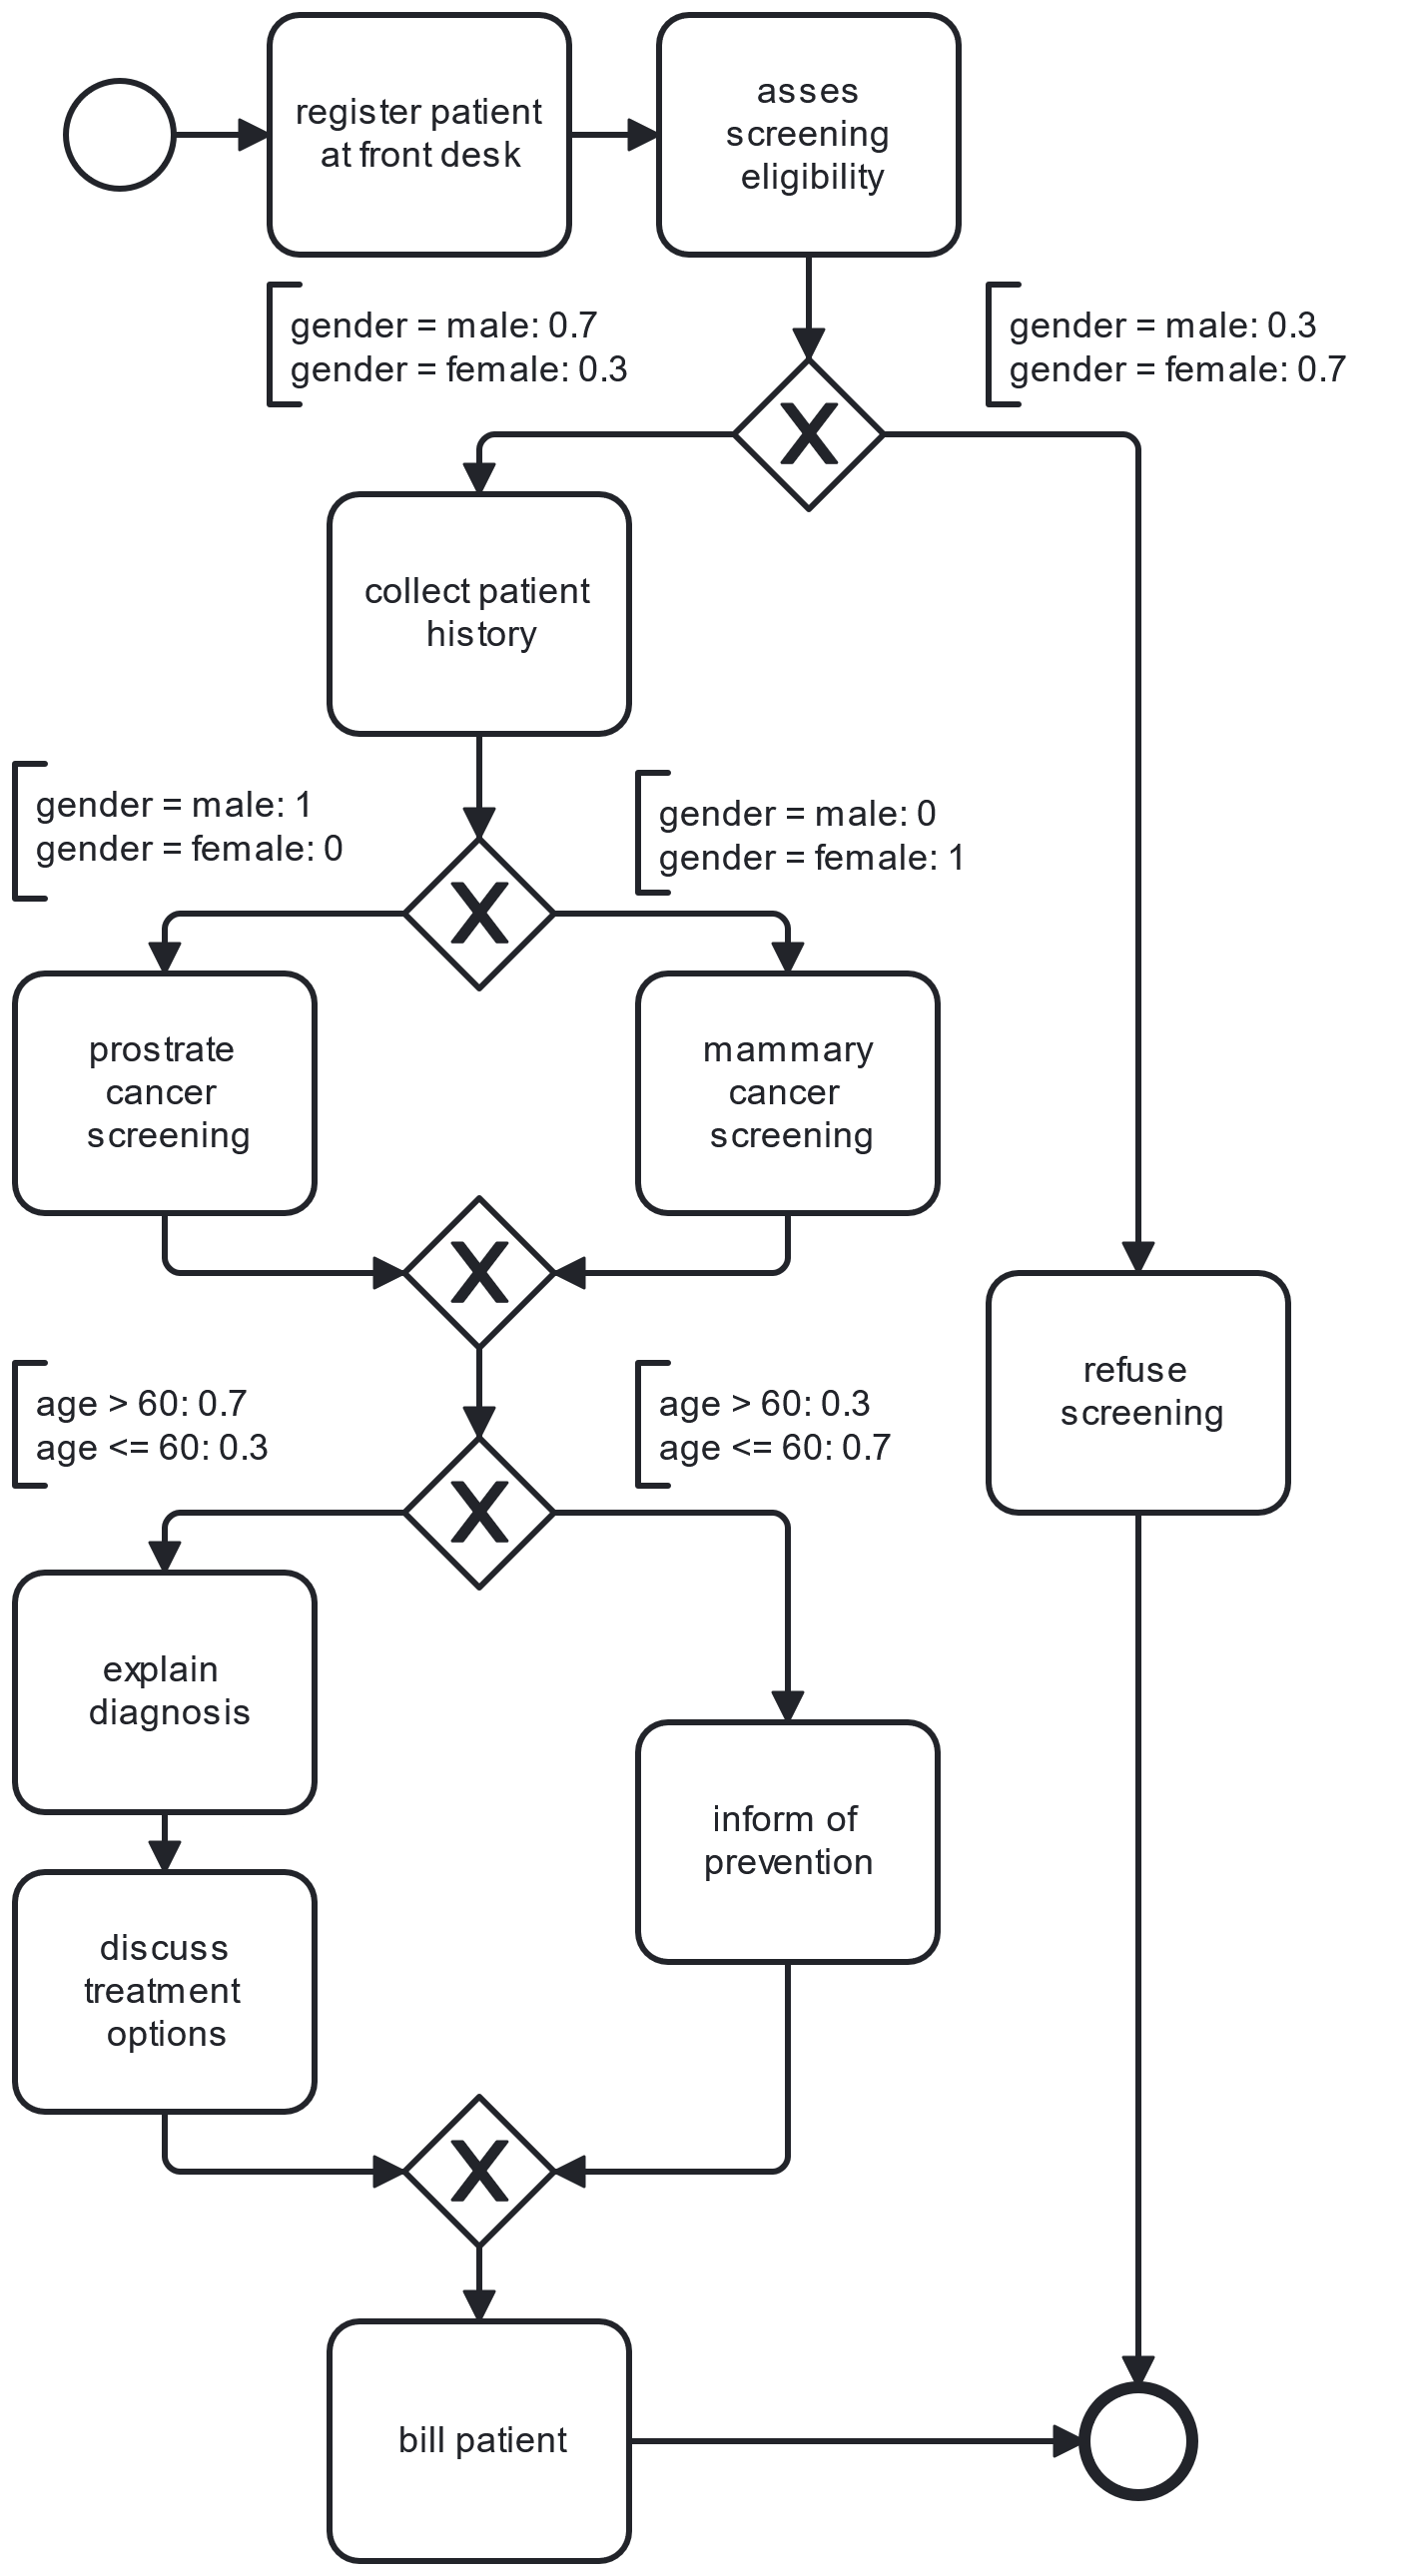
\includegraphics[width=\textwidth,height=0.9\textheight,keepaspectratio]{gfx/cancer_screening.png}
    \caption{This figure shows the BPMN diagram of the process model used for simulating the cancer screening event log.
            The branches of the gateways are annotated with the underlying conditions based on the case attribute values and their corresponding probabilities.}
    \label{fig:cancer_screening}
\end{figure}

\section{Hospital Billing}

%TODO: img of DFG

%TODO: img of age/gender distribution

\section{BPI Challenge 2012}

\begin{figure}[h!]
    \centering
    \begin{minipage}{0.49\textwidth}
        \centering
        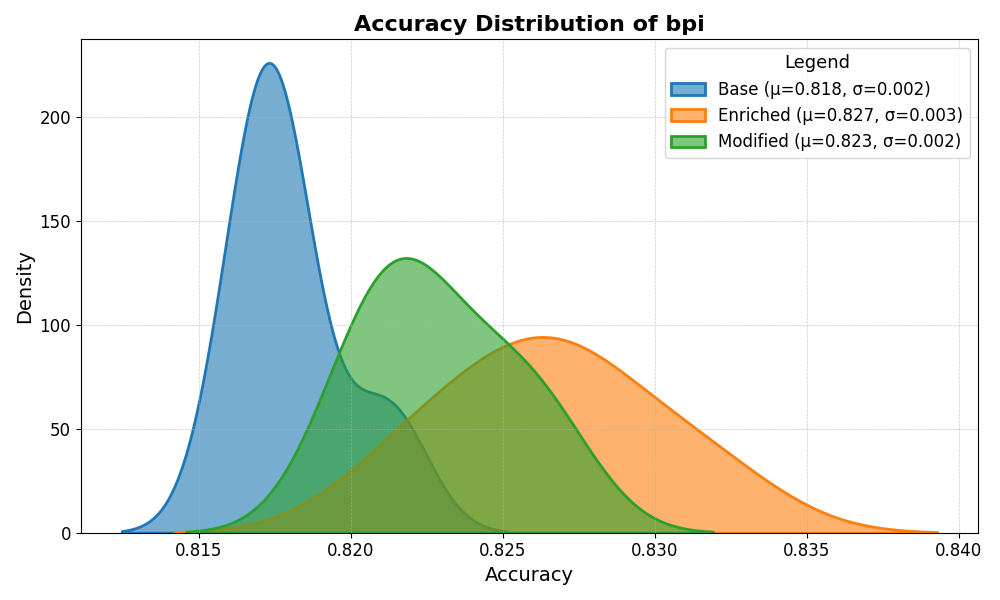
\includegraphics[width=\textwidth]{gfx/bpi_accuracy.png}
        \textbf{(a)}
    \end{minipage}
    \hfill
    \begin{minipage}{0.49\textwidth}
        \centering
        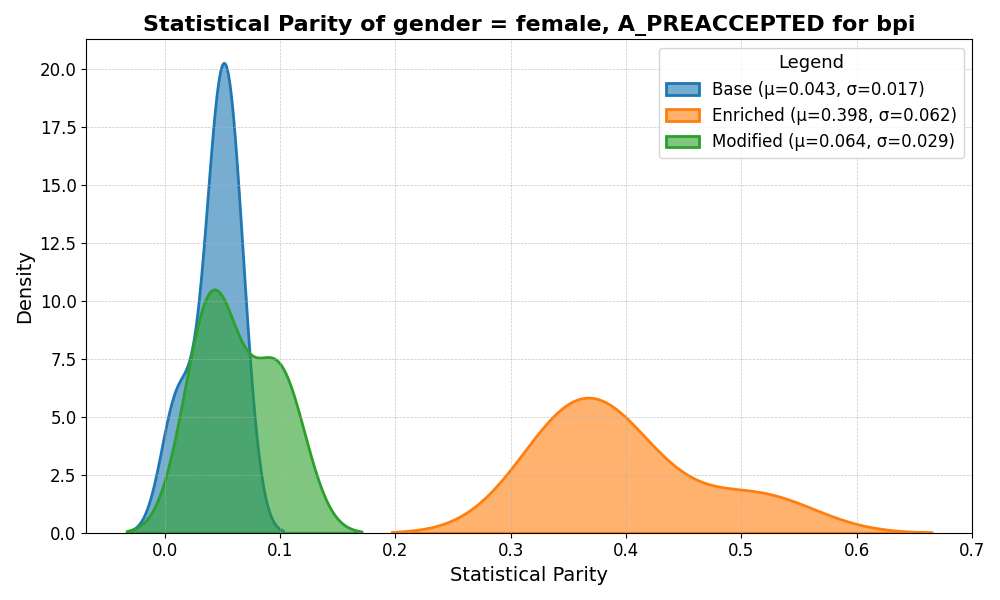
\includegraphics[width=\textwidth]{gfx/bpi_fairness.png}
        \textbf{(b)}
    \end{minipage}
    \caption{Impact of varying bias strength on \textbf{(a)} accuracy and \textbf{(b)} demographic parity.}
    \label{fig:ablation_bias_results}
\end{figure}

\section{Discussion}
